% Figura Anexo I: con precios escalonados, cada mitad ajusta solo en parte y el nivel de precios converge despacio
\documentclass[tikz,border=3pt]{standalone}
\usepackage[T1]{fontenc}
\usepackage[utf8]{inputenc}
\usepackage{amsmath}
\usetikzlibrary{arrows.meta,calc,positioning}
\begin{document}
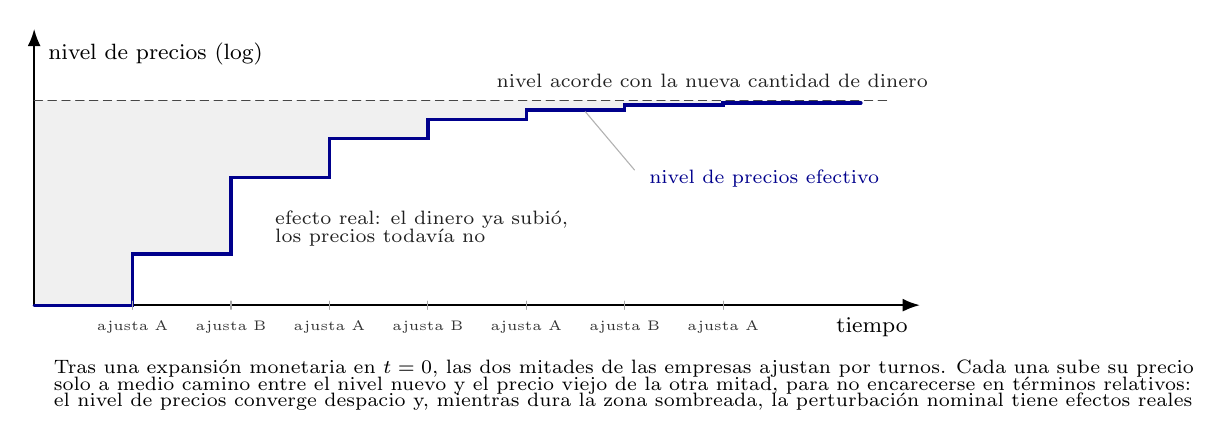
\begin{tikzpicture}[x=1.25cm, y=2.6cm, >={Latex[length=2.2mm]}, line cap=round, font=\footnotesize,
  eje/.style={->, thick},
  guia/.style={densely dashed, gray!80}]
  % Zona del efecto real (entre el nivel coherente y el nivel efectivo)
  \fill[gray!12] (0,0) -- (1,0) -- (1,0.25) -- (2,0.25) -- (2,0.625) -- (3,0.625) -- (3,0.8125) -- (4,0.8125) -- (4,0.90625) -- (5,0.90625) -- (5,0.953) -- (6,0.953) -- (6,0.977) -- (7,0.977) -- (7,0.988) -- (8.4,0.988) -- (8.4,1) -- (0,1) -- cycle;
  \draw[eje] (0,0) -- (9.0,0) node[below left=1pt]{tiempo};
  \draw[eje] (0,0) -- (0,1.35) node[below right=2pt]{nivel de precios (log)};
  % Nivel coherente con la nueva cantidad de dinero
  \draw[densely dashed, gray!55!black] (0,1) -- (8.7,1);
  \node[anchor=south west, font=\scriptsize, gray!25!black] at (4.6,1.015) {nivel acorde con la nueva cantidad de dinero};
  % Escalera del nivel de precios
  \draw[very thick, blue!55!black] (0,0) -- (1,0) -- (1,0.25) -- (2,0.25) -- (2,0.625) -- (3,0.625) -- (3,0.8125) -- (4,0.8125) -- (4,0.90625) -- (5,0.90625) -- (5,0.953) -- (6,0.953) -- (6,0.977) -- (7,0.977) -- (7,0.988) -- (8.4,0.988);
  \node[anchor=west, font=\scriptsize, blue!55!black] at (6.15,0.62) {nivel de precios efectivo};
  \draw[gray!60] (6.1,0.66) -- (5.6,0.945);
  % Turnos de ajuste
  \foreach \x/\g in {1/A,2/B,3/A,4/B,5/A,6/B,7/A}{
    \draw[gray!70] (\x,-0.02) -- (\x,0.02);
    \node[font=\tiny, gray!40!black, anchor=north] at (\x,-0.03) {ajusta \g};
  }
  \node[anchor=west, font=\scriptsize, gray!25!black] at (2.35,0.42) {efecto real: el dinero ya subió,};
  \node[anchor=west, font=\scriptsize, gray!25!black] at (2.35,0.33) {los precios todavía no};
  \node[align=left, anchor=north west, font=\scriptsize] at (0.1,-0.22)
    {Tras una expansión monetaria en $t=0$, las dos mitades de las empresas ajustan por turnos. Cada una sube su precio\\[-2pt]solo a medio camino entre el nivel nuevo y el precio viejo de la otra mitad, para no encarecerse en términos relativos:\\[-2pt]el nivel de precios converge despacio y, mientras dura la zona sombreada, la perturbación nominal tiene efectos reales};
\end{tikzpicture}
\end{document}
